\documentclass[letterpaper]{article}
\usepackage{aaai17}  %Required
\usepackage{times}  %Required
\usepackage{helvet}  %Required
\usepackage{courier}  %Required
\usepackage{url}  %Required
\usepackage{graphicx}  %Required
\frenchspacing  %Required
\setlength{\pdfpagewidth}{8.5in}  %Required
\setlength{\pdfpageheight}{11in}  %Required

% MATHEMATICS
\usepackage{amsmath}
\usepackage{amsfonts}
\usepackage{amssymb}
\usepackage[algoruled, titlenumbered, vlined]{algorithm2e}

% SPACING
\usepackage{xspace}
\usepackage{enumitem}
\setlist{nolistsep}

% COMMENTS
\usepackage{verbatim}

% Definitions
\usepackage{./definitions}

\setcounter{secnumdepth}{2}

% GRAPHICS
%\usepackage[]{graphicx}
%\usepackage{caption}
\usepackage{subcaption}
\usepackage{multicol}

% Graphics Path
\graphicspath{{./images/}}

\pdfinfo{
  /Title (Analytic Decision Analysis via Symbolic Dynamic Programming for Parameterized Hybrid MDPs)
  /Author (Shamin Kinathil, Harold Soh, Scott Sanner)
}

\begin{document}
    
%--------------------------------------------------------------------------------------------------
% Front Matter
%--------------------------------------------------------------------------------------------------
\title{Analytic Decision Analysis via Symbolic Dynamic Programming for Parameterized Hybrid MDPs}

\author{Shamin Kinathil \\
    ANU and Data61, CSIRO \\
    Canberra, ACT, Australia \\
    shamin.kinathil@anu.edu.au \\
    \And
    Harold Soh \\
    University of Toronto \\
    Toronto, ON, Canada \\
    harold.soh@utoronto.ca \\
    \And
    Scott Sanner  \\
    University of Toronto \\
    Toronto, ON, Canada \\
    ssanner@mie.utoronto.ca \\
}
\maketitle

\begin{abstract}
    
    Decision analysis w.r.t. unknown parameters is a critical task in decision-making under uncertainty.  For example, we may need to (i) perform inverse learning of the cost parameters of a multi-objective reward based on observed agent behavior; (ii) perform sensitivity analyses of policies to various parameter settings; or (iii) analyze and optimize policy performance as a function of policy parameters. When such problems have mixed discrete and continuous state and/or action spaces, this leads to parameterized hybrid MDPs (PHMDPs) that are often approximately solved via discretization, sampling, and/or local gradient methods (when optimization is involved). In this paper we combine two recent advances that allow for the first exact solution and optimization of PHMDPs. We first show how each of the aforementioned use cases can be formalized as PHMDPs, which can then be solved via an extension of symbolic dynamic programming (SDP) even when the solution is piecewise nonlinear. Secondly, we can leverage recent advances in non-convex solvers that require symbolic forms of the objective function for non-convex global optimization in (i), (ii), and (iii) using SDP to derive symbolic solutions for each PHMDP formalization. We demonstrate the efficacy and scalability of our optimal analytical framework on nonlinear examples of each of the aforementioned use cases.
    
\end{abstract}

%--------------------------------------------------------------------------------------------------
% Body
%--------------------------------------------------------------------------------------------------

\section{Introduction}
\label{sec:introduction}

Markov Decision Processes (MDPs) are the de facto standard framework for decision theoretic planning in fully observable environments~\cite{Boutilier_JAIR_1999}. Traditional MDP solution techniques often assume that the parameters of the model are known. However, in practice, model parameters are usually estimated from limited data or elicited from humans and are naturally uncertain. Hence decision analysis w.r.t. unknown parameters is a critical task in decision-making under uncertainty with applications to: (i) inverse learning of parameters of multi-objective rewards; (ii) sensitivity analyses of policies to various parameter settings; and (iii) analyzing and optimizing policy performance as a function of policy parameters. Formalizing models to address each of the aforementioned use cases is often fraught, due to the specification leading to hybrid (mixed discrete and continuous state and/or action) MDPs with nonlinear and/or piecewise structure that have been traditionally very difficult to solve.

In this paper we make the following key contributions:
\begin{itemize}
    \item We present {\it Parameterized Hybrid MDPs} (PHMDPs) as a unified model of the aforementioned use cases and provide an algorithm that solves PHMDPs exactly and in closed-form by defining a parameterized variant of Symbolic Dynamic Programming (SDP)~\cite{Boutilier_IJCAI_2001} extended to hybrid MDPs~\cite{Sanner_UAI_2011}. 
    %\item We use the PHMDP framework in conjunction with parameterized SDP to 
    \item We provide the \textit{first} completely symbolic encodings of the aforementioned use cases, which in turn enables the use of recent advances in symbolic non-convex optimization techniques with \textit{guarantees}~\cite{Gao2013}.
    \item We present the \textit{first exact} symbolic analysis of vaccination policies in an SIR epidemiological model~\cite{KermackMcKendrick_1927}, as well exact solutions to the inverse learning of parameters in a multi-objective reward domain and sensitivity analyses of portfolio execution strategies.
\end{itemize}

\section{Related Work}
\label{sec:background}

In this section we briefly survey prior art in the areas of multi-objective reasoning, exact sensitivity analysis and nonlinear parameterized policy optimization and conclude with a discussion of alternate uses of the term \emph{parameterized} in the MDP literature that contrasts with our work.

The techniques used to solve Multi-objective MDPs (MOMDPs) with unknown preferences depend on the nature of the scalarization function used to weight each reward component~\cite{Roijers_JAIR_2013}. Methods such as the Convex Hull Value Iteration algorithm~\cite{Barrett_ICML_2008} can be used for discrete \emph{enumerated state} MOMDPs with any linear preference function. Nonlinear scalarization functions require the calculation of the Pareto front, which can be prohibitively large. As a result, Pareto front approximation techniques such as those of ~\cite{Chatterjee_STACS_2006} and~\cite{Pirotta_AAAI_2015} or Lorenz optimal refinements such as~\cite{Perny_AAAI_2013} are often used. In this work we present the first exact \emph{factored hybrid} MOMDP solutions as a symbolic function of multiobjective weights via PHMDPs and SDP.
%the framework of PHMDPs and SDP.

To date, most research into sensitivity analysis of MDP parameters has focused on uncertainty within the specification of the transition function~\cite{Kalyanasundaram_AJC_2004}, reward function~\cite{Tan_JAP_2011}, or a combination of both~\cite{Givan_AI_2000}, in discrete MDPs. The framework that we introduce in this paper enables \textit{exact} sensitivity analysis for PHMDPs that allows it to be applied in continuous state settings and permits the derivation and analysis of the \emph{optimal} policy as a symbolic function of these parameters.

Policy gradient methods rely upon optimizing parameterized policies with respect to the expected return by gradient descent. 
Two of the most prominent approaches have been the finite-difference methods, such as those of~\cite{Ng_UAI_2000}, and Monte Carlo methods, such as~\cite{Sutton_NIPS_1999,Baxter_ISCAS_2000}, both of which only converge to local optima.
%are numerically oriented and sample based. 
Our use of PHMDPs and SDP allows us to solve for a globally optimal policy as a parameterized function of policy parameters.

Finally, as a point of differentiation from other uses of the term \emph{parameterized} in the MDP literature, we remark that other works~\cite{Doshi-VelezK16,Duff_UMA_2002,Dearden_UAI_1999,Gopalan_COLT_2015} have used Parameterized MDP to refer to MDPs with latent parameters whose beliefs can be updated by observing reward and transition samples. In contrast, in this work we assume strict uncertainty of continuous MDP parameters in models that are otherwise fully specified; in this way we can treat parameters simply as free variables that can be parametrically analyzed via recent advances in symbolic solution methods and non-convex optimizers~\cite{Gao2013}.

\section{Parameterized Hybrid MDPs}
\label{sec:hybrid_mdps}

In this section we introduce PHMDPs.
%In this section we introduce Parameterized Hybrid Markov Decision Processes (PHMDPs).

\subsection{Definition}
\label{sec:phmdp_def}

A parameterized hybrid Markov Decision Process (PHMDP) is defined by the tuple {\footnotesize \PMDPTuple}. {\footnotesize \State} specifies a vector of states given by {\footnotesize $(\vec{d}, \vec{x}) =  \left( d_1, \ldots, d_m, x_1, \ldots, x_n \right) $}, where each {\footnotesize $ d_i \in \left\lbrace 0, 1 \right\rbrace $} {\footnotesize $\left( 1 \leq i \leq m \right)$} is discrete and each {\footnotesize$ x_j \in \Real $} {\footnotesize $\left( 1 \leq j \leq   n \right)$} is continuous. {\footnotesize $\Action^{h}_{s}$} specifies a finite set of state and horizon dependent actions.  {\footnotesize $\vec{\theta} $} are free parameters from the parameter space {\footnotesize $ \Theta $}. PHMDPs are naturally factored~\cite{Boutilier_JAIR_1999} in terms of the state variables {\footnotesize$\vec{d}$} and {\footnotesize $\vec{x}$}. Hence, the joint transition model can be written as:
{\footnotesize
%    \abovedisplayskip=0pt
%    \belowdisplayskip=0pt
    \begin{align}
    \label{eq:hmdp_tfunc}
    \Transition :& \, \ProbArg{ \left. \vec{d}', \vec{x}' \middle| \vec{d}, \vec{x}, a, \vec{\theta} \right.} = \nonumber \\
    & \prod_{i=1}^{m} \ProbArg{ \left. d_i' \middle| \vec{d}, \vec{x}, a, \vec{\theta} \right. } \prod_{j=1}^{n} \ProbArg{ \left. x_j' \middle| \vec{d}, \vec{d}', \vec{x}, a, \vec{\theta} \right. },
    \end{align}   
}
where {\footnotesize $ a \in \Action^{h}_{s} $}. The transition model permits discrete noise in the sense that {\footnotesize $ \ProbArg{ x_j' | \vec{d}, \vec{d}', \vec{x}, a, \vec{\theta} } $} may condition on $ \vec{d}' $, which are stochastically sampled according to their conditional probability functions. We note that this framework can be extended to Dynamic Bayesian Networks with arbitrary intermediate variable layers that allow one to emulate synchronic arc dependencies and relax the discrete and continuous stratifications.

{\footnotesize \RewardFunc} is the reward function which encodes the preferences of the agent. {\footnotesize \Horizon} represents the number of decision steps until termination and the discount factor {\footnotesize $\gamma \in [0, 1)$} is used to geometrically discount future rewards. A policy {\footnotesize $\pi : \State \times \Horizon \times \vec{\theta} \rightarrow \Action$}, specifies the action to take in every state and horizon. The value function of the optimal policy {\footnotesize$ \pi^{*} $} satisfies:
{\footnotesize 
%    \abovedisplayskip=0pt
%    \belowdisplayskip=0pt
    \begin{align}
    \label{eq:opt_vfunc}
    V^{\pi^{*}}\left(\vec{d}, \vec{x}; \vec{\theta}\right) &= \max_{a \in \Action} \left\{ Q^{\pi}\left(\vec{d}, \vec{x}, a; \vec{\theta}\right) \right\}.
    \end{align}
}%
{\footnotesize $ Q^{\pi}\left(\vec{d}, \vec{x}, a; \vec{\theta}\right) $} gives the expected return starting from state {\footnotesize $(\vec{d}, \vec{x}) \in \State$}, taking action {\footnotesize $ a \in \Action^{h}_{s} $}, and then following policy $ \pi $. In general, an agent's objective is to find an optimal policy {\footnotesize$ \pi^{*} $} which maximises the expected sum of discounted rewards over horizon {\footnotesize \Horizon}\footnote{All of the code can be found at \url{https://github.com/skindev/xadd-inference-1/src/cmomdp}.}. 
We again remark that in our formulation of PHMDPs {\footnotesize $ \vec{\theta} $} are free parameters and not learned from reward and transition samples.

\section{Parameterized Symbolic Dynamic Programming}
\label{sec:sdp}

Symbolic Dynamic Programming (SDP)~\cite{Boutilier_IJCAI_2001} is the process of performing dynamic programming via symbolic manipulation. In the following sections we present a brief overview of SDP operations and how it can be adapted to solve PHMDPs.
%Parameterized Hybrid MDPs.

\subsection{Symbolic Case Calculus}

SDP assumes that all functions can be represented in case statement form~\cite{Boutilier_IJCAI_2001}:
{\footnotesize 
%    \abovedisplayskip=5pt
%    \belowdisplayskip=0pt
    \begin{align*}
    f = 
    \begin{cases}
    \phi_1: & f_1 \\ 
    \vdots & \vdots\\ 
    \phi_k: & f_k \\ 
    \end{cases}
    \end{align*}
}%

Here, {\footnotesize$ f_i $} are nonlinear expressions over {\footnotesize$( \vec{d}, \vec{x}, \vec{\theta})$} and {\footnotesize$\phi_i$} are logical formulae defined over {\footnotesize$( \vec{d}, \vec{x}, \vec{\theta})$} that can consist of arbitrary logical combinations of tests on {\footnotesize$\vec{d}$} and inequalities {\footnotesize$\left( \geq, >, <, \leq \right)$} over nonlinear expressions of   {\footnotesize$(\vec{x}, \vec{\theta})$}. We assume that the set of conditions {\footnotesize$\left\lbrace \phi_1, \ldots, \phi_k \right\rbrace$} disjointly and exhaustively partition {\footnotesize$(\vec{d}, \vec{x}, \vec{\theta})$} such that {\footnotesize$f$} is well-defined for all {\footnotesize$(\vec{d}, \vec{x}, \vec{\theta})$}. Henceforth, we refer to functions with linear {\footnotesize$\phi_i$} and piecewise linear {\footnotesize$f_i$} as linear piecewise linear (LPWL) and functions with nonlinear {\footnotesize$\phi_i$} and piecewise nonlinear {\footnotesize$f_i$} as nonlinear piecewise nonlinear (NPWN) functions.

Operations on case statements may be either unary or binary. Unary operations on a single case statement \emph{f}, such as scalar multiplication {\footnotesize$c \cdot f$} where {\footnotesize$ c \in \mathbb{R} $}, are applied to  each {\footnotesize$f_i \left(1 \leq i \leq k\right)$}. Binary operations such as addition, subtraction and multiplication are executed in two stages. Firstly, the cross-product of the logical partitions of each case statement is taken, producing paired partitions. Finally, the binary operation is applied to the resulting paired partitions. The ``cross-sum'' {\footnotesize$\oplus$} operation can be performed on two cases: 
{\footnotesize 
%        \abovedisplayskip=5pt
    %    \belowdisplayskip=0pt
    \begin{center}
        \begin{tabular}{r c c c l}
            $\begin{cases}
            \phi_1: \hspace{-1mm} & \hspace{-1mm} f_1  \\ 
            \phi_2: \hspace{-1mm} & \hspace{-1mm} f_2  \\ 
            \end{cases}$
            $\oplus$
            &
            \hspace{-4mm}
            $\begin{cases}
            \psi_1: \hspace{-1mm} & \hspace{-1mm} g_1  \\ 
            \psi_2: \hspace{-1mm} & \hspace{-1mm} g_2  \\ 
            \end{cases}$
            &
            \hspace{-4mm} 
            $ = $
            &
            \hspace{-4mm}
            $\begin{cases}
            \phi_1 \wedge \psi_1: & f_1 + g_1 \\
            \phi_1 \wedge \psi_2: & f_1 + g_2 \\
            \phi_2 \wedge \psi_1: & f_2 + g_1 \\
            \phi_2 \wedge \psi_2: & f_2 + g_2  \\
            \end{cases}$
        \end{tabular}
    \end{center}
}%
%\vspace{-4em}

``cross-subtraction'' {\footnotesize$\ominus$} and ``cross-multiplication'' {\footnotesize$\otimes$} are defined in a similar manner but with the addition operator replaced by the subtraction and multiplication operators, respectively. Some partitions resulting from case operators may be inconsistent and are thus removed. All of the operations presented thus far are closed-form for NPWN functions~\cite{Sanner_UAI_2011}.

A case statement can be maximized with respect to a continuous parameter {\footnotesize$y$} as {\footnotesize $ f_1(\vec{x}) = \contmax_{y}f_2(\vec{x}, y) $}. Continuous maximization is used for continuous {\footnotesize $\Action$} PHDMPs and is closed-form for LPWL functions; maximization of discrete {\footnotesize $\Action$} remains closed-form for all NPWN functions. We refer the reader to~\cite{Sanner_UAI_2011,Zamani_AAAI_2012} for more details. %expositions of SDP.% for piecewise continuous functions.

In principle, case statements can be used to represent all PHMDP components. In practice, case statements are implemented using a more compact representation known as Extended Algebraic Decision Diagrams (XADDs)~\cite{Sanner_UAI_2011}, which also support efficient versions of all of the aforementioned operations. 

\subsection{SDP for Parameterized Hybrid MDPs}

Value iteration (VI)~\cite{Bellman_PU_1957} can be modified to solve PHMDPs in terms of the following case operations:
{\footnotesize 
%    \abovedisplayskip=0pt
%    \belowdisplayskip=0pt
    \begin{align}
    Q^{h} \left( \vec{d}, \vec{x}, a; \vec{\theta} \right) = \Reward \left( \vec{d}, \vec{x}, a; \vec{\theta} \right) \oplus \gamma \qquad \qquad \qquad \qquad &  \nonumber \\ 
    \bigoplus_{\vec{d}'} \int_{\vec{x}'} \ProbArg{ \left. \vec{d}', \vec{x}' \middle| \vec{d}, \vec{x}, a; \vec{\theta} \right.} \otimes V^{h-1} \left( \vec{d}', \vec{x}'; \vec{\theta} \right) \, d\vec{x}' & \label{eq:vi_sdp_qfunc} \\
    V^{h}\left( \vec{d}, \vec{x}; \vec{\theta} \right) = \casemax_{a \in \mathcal{A}} \left\{ Q^{h} \left( \vec{d}, \vec{x}, a; \vec{\theta} \right) \right\} \qquad \qquad & \label{eq:vi_sdp_vfunc}
    \end{align}
}%

{\footnotesize $\ProbArg{\left. \vec{d}', \vec{x}' \middle| \vec{d}, \vec{x}, a; \vec{\theta} \right.}$ } is specified in Equation~\eqref{eq:hmdp_tfunc}. The parameters {\footnotesize $\theta_i$} are stationary free variables and hence do not change during the backup operation. Continuous state parameters {\footnotesize $ \vec{x} $} are handled in a similar fashion. Symbolic integration over continuous variables are carried out with respect to a deterministic Dirac {\footnotesize $\delta$} function. This is a consequence of the discrete noise restriction mentioned in section~\ref{sec:phmdp_def} and yields a closed-form backup operation even with NPWN {\footnotesize $\Transition$} or {\footnotesize $\Reward$} components~\cite{Sanner_UAI_2011}. 

A particular strength of SDP is that all operations will automatically condition the value and policy on the {\footnotesize $\theta_i$}, without needing to know their value a priori, yielding the parameterized value function in Equation~\eqref{eq:vi_sdp_vfunc}.

In the case of discrete {\footnotesize \Action} it can be proved that all of the SDP operations used in Equations~\eqref{eq:vi_sdp_qfunc} and~\eqref{eq:vi_sdp_vfunc} are closed-form for NPWN functions~\cite{Sanner_UAI_2011}. In the case of continuous {\footnotesize \Action} all of the operations are closed-form for only LPWL functions~\cite{Zamani_AAAI_2012}.

\subsubsection{Inverse Learning for Multi-objective PHMDPs}

A possible formulation for the inverse learning problem for multi-objective MDPs is to constrain the Q-values corresponding to the observed behavior and maximize {\footnotesize $\vec{\theta}$}, which can be interpreted as multi-objective weights that best explain the observed behavior: 
\begin{align}
\label{eq:irl_q}
\max_{\vec{\theta}} \max_{a_k, a_k \neq \pi } Q^{h} \left(\vec{d}, x, a_k; \vec{\theta} \right) \ominus Q^{h} \left(\vec{d}, x, a_{-k}; \vec{\theta} \right),
\end{align}
where {\footnotesize $ x $} can either be fixed or a region specified in the constraints, {\footnotesize $a_{k}$} refers to the action taken under the policy {\footnotesize $\pi$} in a particular state and {\footnotesize $a_{-k}$} refers to all other available actions in that state. 
%We note that this formulation is but one of many possible approaches to inverse reinforcement learning and refer the reader to~\cite{Ng_ICML_2000} for alternate approaches. 
We note that Equation~\eqref{eq:irl_q} is one of many possible formulations to inverse reinforcement learning and refer the reader to~\cite{Ng_ICML_2000} for alternate approaches. 

\subsubsection{Sensitivity Analysis for PHMDPs}

Sensitivity analysis for PHMDPs can be analysed exactly and in closed-form via SDP by first calculating Equation~\eqref{eq:vi_sdp_vfunc} and then taking symbolic derivatives, up to any order, with respect to %the parameter 
{\footnotesize $\vec{\theta}$}.

\subsubsection{Nonlinear Parameterized Policy Optimization Methods for PHMDPs}

Parameterized policies {\footnotesize $ \pi(\vec{\theta}) $} for PHMDPs, where {\footnotesize $\vec{\theta}$} may be nonlinear, can be analyzed exactly and in closed-form via SDP by substituting {\footnotesize $ \pi(\vec{\theta}) $} in for {\footnotesize  $ a $} in Equation~\eqref{eq:vi_sdp_qfunc}. This precludes the need for action maximization in Equation~\eqref{eq:vi_sdp_vfunc} and makes SDP efficient in both computation time and space. The parametric nature of this function allows us to directly apply non-convex optimization tools that require symbolic forms of the objective function. This yields a global optimization of the function in contrast to policy gradient methods which only guarantee local optimization.

\section{Results}
\label{sec:results}

In this section we demonstrate the efficacy and tractability of PHMDPs by calculating the first known optimal solutions to three difficult nonlinear sequential decision problems. We note that while dOp~\cite{Gao2013} offers strong {\footnotesize $ \delta $}-optimality guarantees, we found that nonlinear solvers such as $ \mathtt{fmincon} $~\cite{MATLAB_2010}, an interior-point algorithm, perform comparably well and are much more efficient, hence we use $ \mathtt{fmincon} $.

\subsection{Inverse Learning for Navigation}
\label{sec:results_navigation}

The domain is specified as follows: {\footnotesize $ \State = \left\langle loc \right\rangle$}, where $ loc $ is the location of the vehicle. {\footnotesize $ \Action \in \left\lbrace 0.0, 5.0 \right\rbrace $} is the amount by which vehicle moves relative to its current location. {\footnotesize $ \Transition\left( loc' | loc, a \right) = \delta \left[ loc' - (loc + a) \right] $}, where {\footnotesize $ a \in \Action $}. {\footnotesize $ \Reward\left(\vec{w}, loc, loc'\right) = w_1 \cdot \Reward_{\mathtt{region}} + w_2 \cdot \Reward_{\mathtt{move}} $} where,

{\footnotesize 
%    \abovedisplayskip=10pt
%    \belowdisplayskip=0pt
%    \renewcommand{\arraystretch}{1.5}
    \begin{tabular}{ll}    
        $ \Reward_{\mathtt{region}}(loc') = $ &  $ \Reward_{\mathtt{move}}(loc, loc') =  $ \\
        \qquad $ \begin{cases}
        (loc' \geq 10.0 ) : 				& loc' \\
        \text{otherwise} : 					& 0.0 \\
        \end{cases} $ 						& \qquad $ - \lvert loc' - loc \rvert  $\\
        %        $ \Reward_{\mathtt{move}}(loc, loc') = - (loc' - loc)$ & $ $ \\                        
    \end{tabular}
} 

Figure~\ref{fig:navigation_vf} shows the optimal value function at {\footnotesize$ \Horizon = 15 $} and reveals the trade-off between reaching the goal region and incurring a movement cost {\footnotesize $w_2 \cdot \Reward_{\mathtt{move}}$}, when {\footnotesize $w_2 \in [0.0, 50.0]$}. The vehicle will incur the movement cost as long as it is mitigated by the {\footnotesize $ \Reward_{\mathtt{region}}$} reward. Furthermore, the range of acceptable non-zero movement costs decreases the further the vehicle is from the goal region. 
%For example, when {\footnotesize $loc = -20.0$} the vehicle will only move if the cost is close to {\footnotesize $0.0$}, whereas when the {\footnotesize $loc = 0.0$}, the vehicle is willing to incur higher movement costs. 
In Figure~\ref{fig:navigation_opt} we utilise Equation~\eqref{eq:irl_q} to learn the parameters (weights) of the multi-objective reward under the following sub-optimal policy: {\footnotesize $ \tilde{\pi}(0 < loc < 10) = 5.0,  \tilde{\pi}(loc < 0 \,\mathrm{or}\, loc > 10) = 0.0$}. We observe that when {\footnotesize $a = 0.0$}, {\footnotesize $ w_2 = 50.0$}, its maximum value. When {\footnotesize $a = 5.0$}, there are two different gradients for {\footnotesize $ w_2 $}, one when {\footnotesize $ (0 < loc < 5) $} and another when {\footnotesize $ (5 < loc < 10) $}. 
%The steepness of the gradient in the latter region illustrates that being one step closer to the goal region allows the vehicle to accumulate an additional goal region reward over the finite horizon.
The steeper gradient in the latter region indicates that being one step closer to the goal region allows the vehicle to accumulate an additional {\footnotesize $ \Reward_{\mathtt{region}}$} reward over {\footnotesize$ \Horizon $}.

{\centering
    \begin{figure}[]
        \begin{tabular}{cc}
            \begin{subfigure}{0.45\columnwidth}
                \centering
                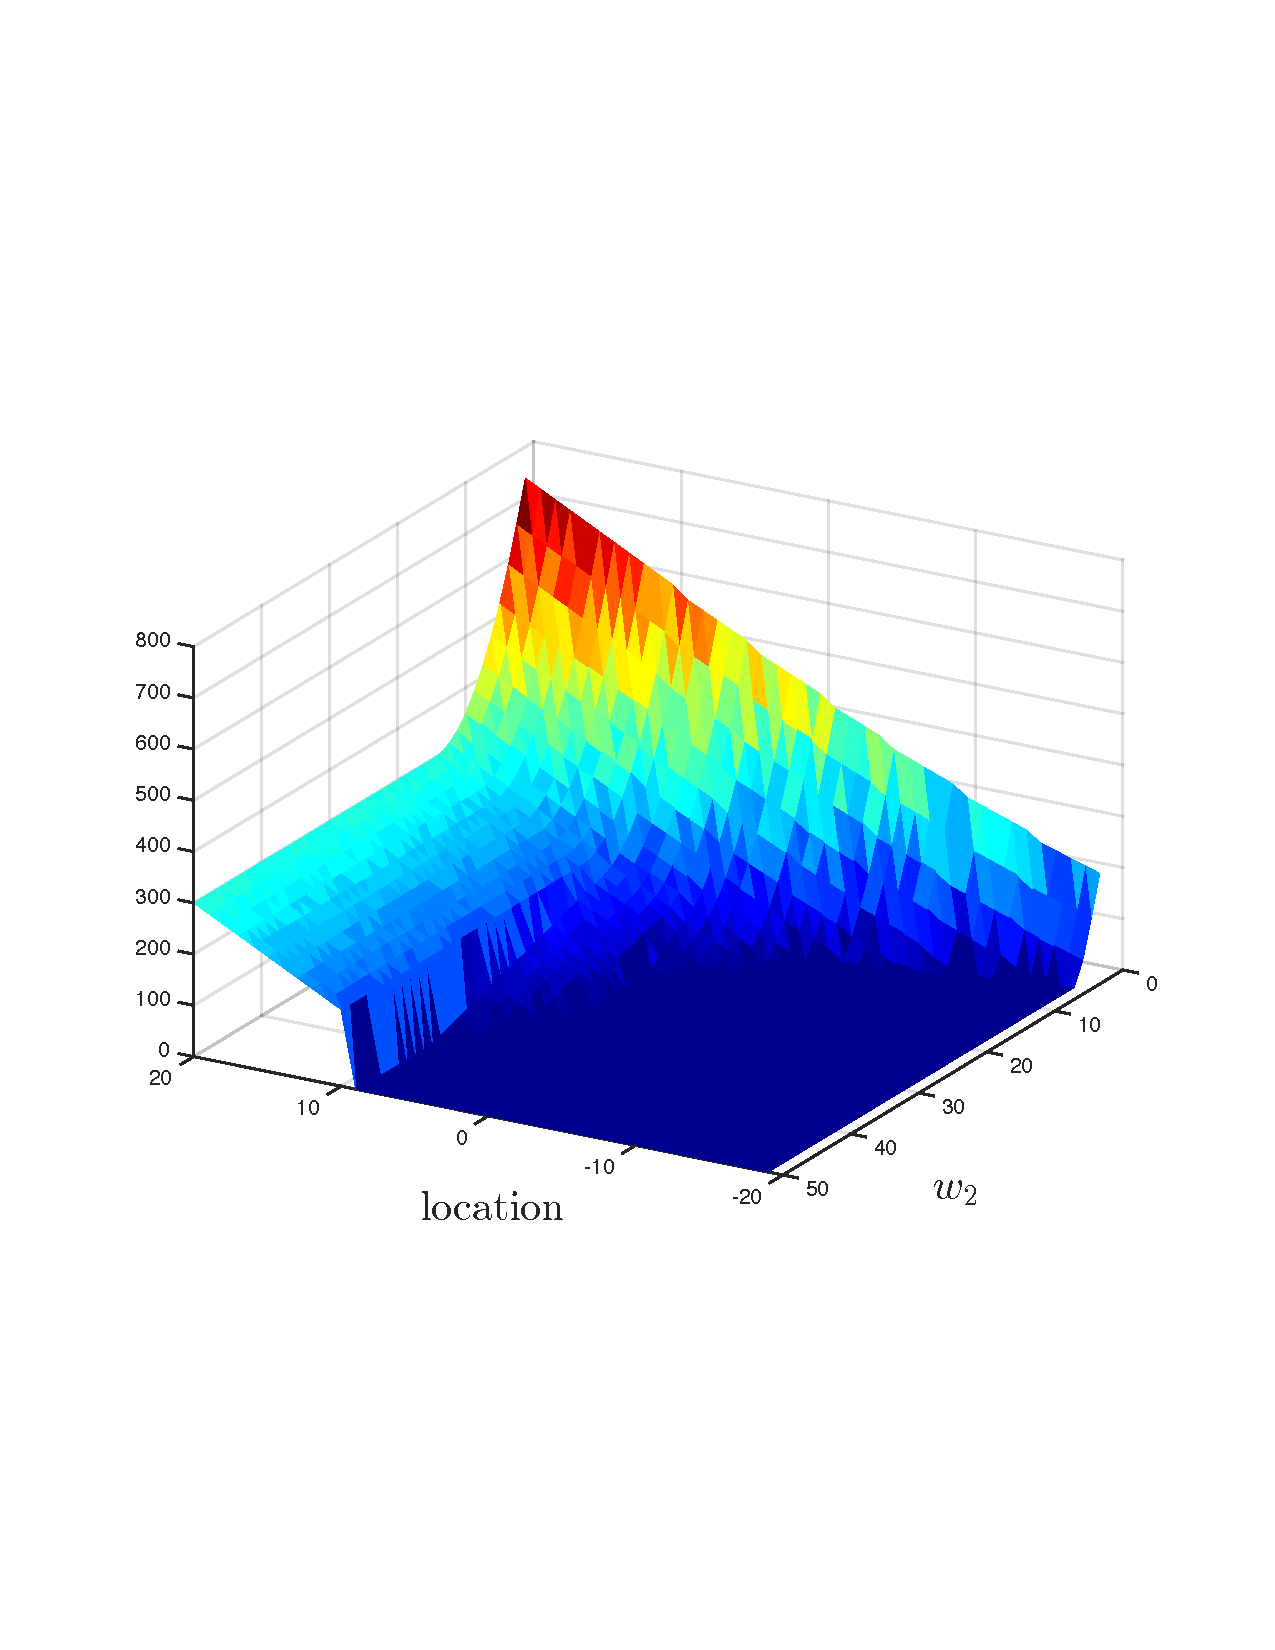
\includegraphics[width=\textwidth]{images/robot_vf_new}
                \caption{{\footnotesize $V^{\pi^{*}}(loc, w_2; w_1 = 1.0)$}}
                \label{fig:navigation_vf}
            \end{subfigure} &
            \begin{subfigure}{0.45\columnwidth}
                \centering
                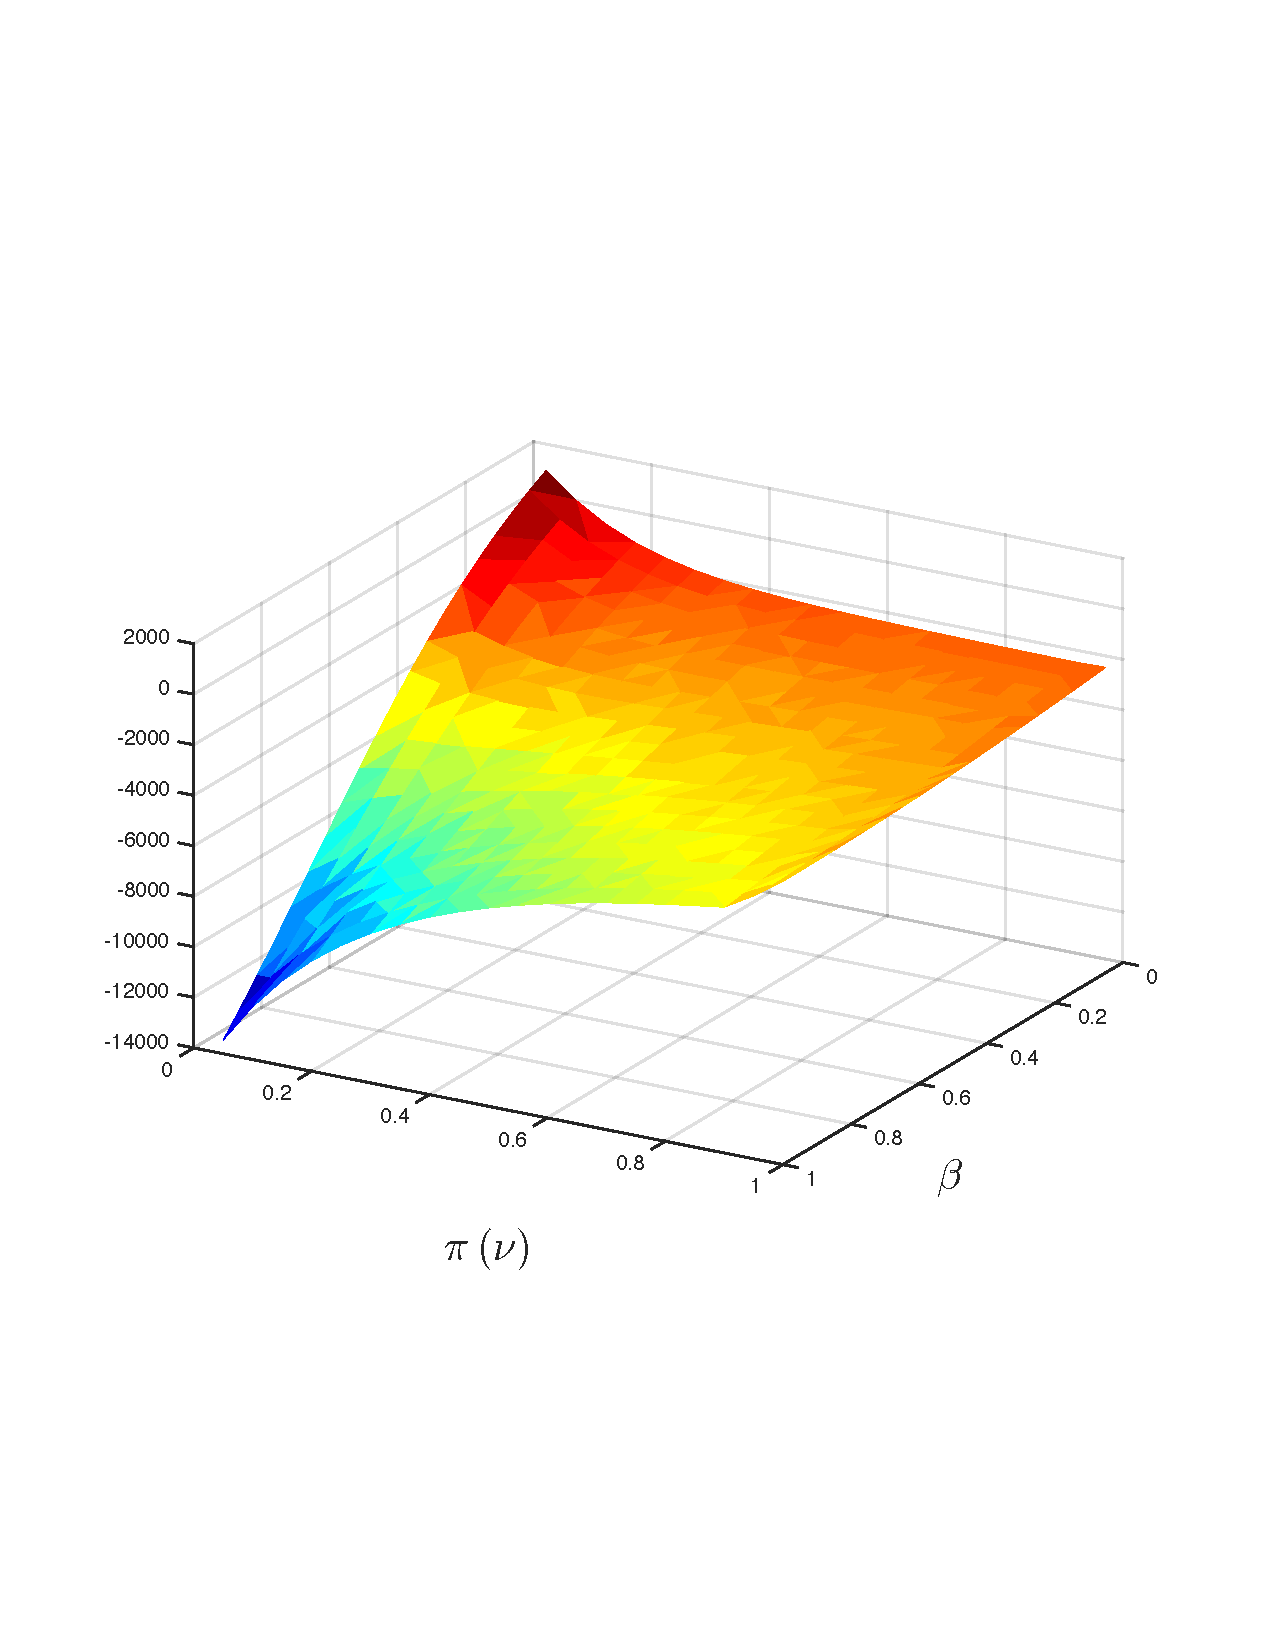
\includegraphics[width=\textwidth]{images/sir_vf_new}
                \caption{{\footnotesize $V^{\pi^{*}}(\beta, \nu; s, i, r, \lambda, \\\hspace{\textwidth}\qquad cost_{\mathtt{inf}}, cost_{\mathtt{vaccine}})$}}
                \label{fig:sir_vf}
            \end{subfigure}
            \\
            \begin{subfigure}{0.45\columnwidth}
                \centering
                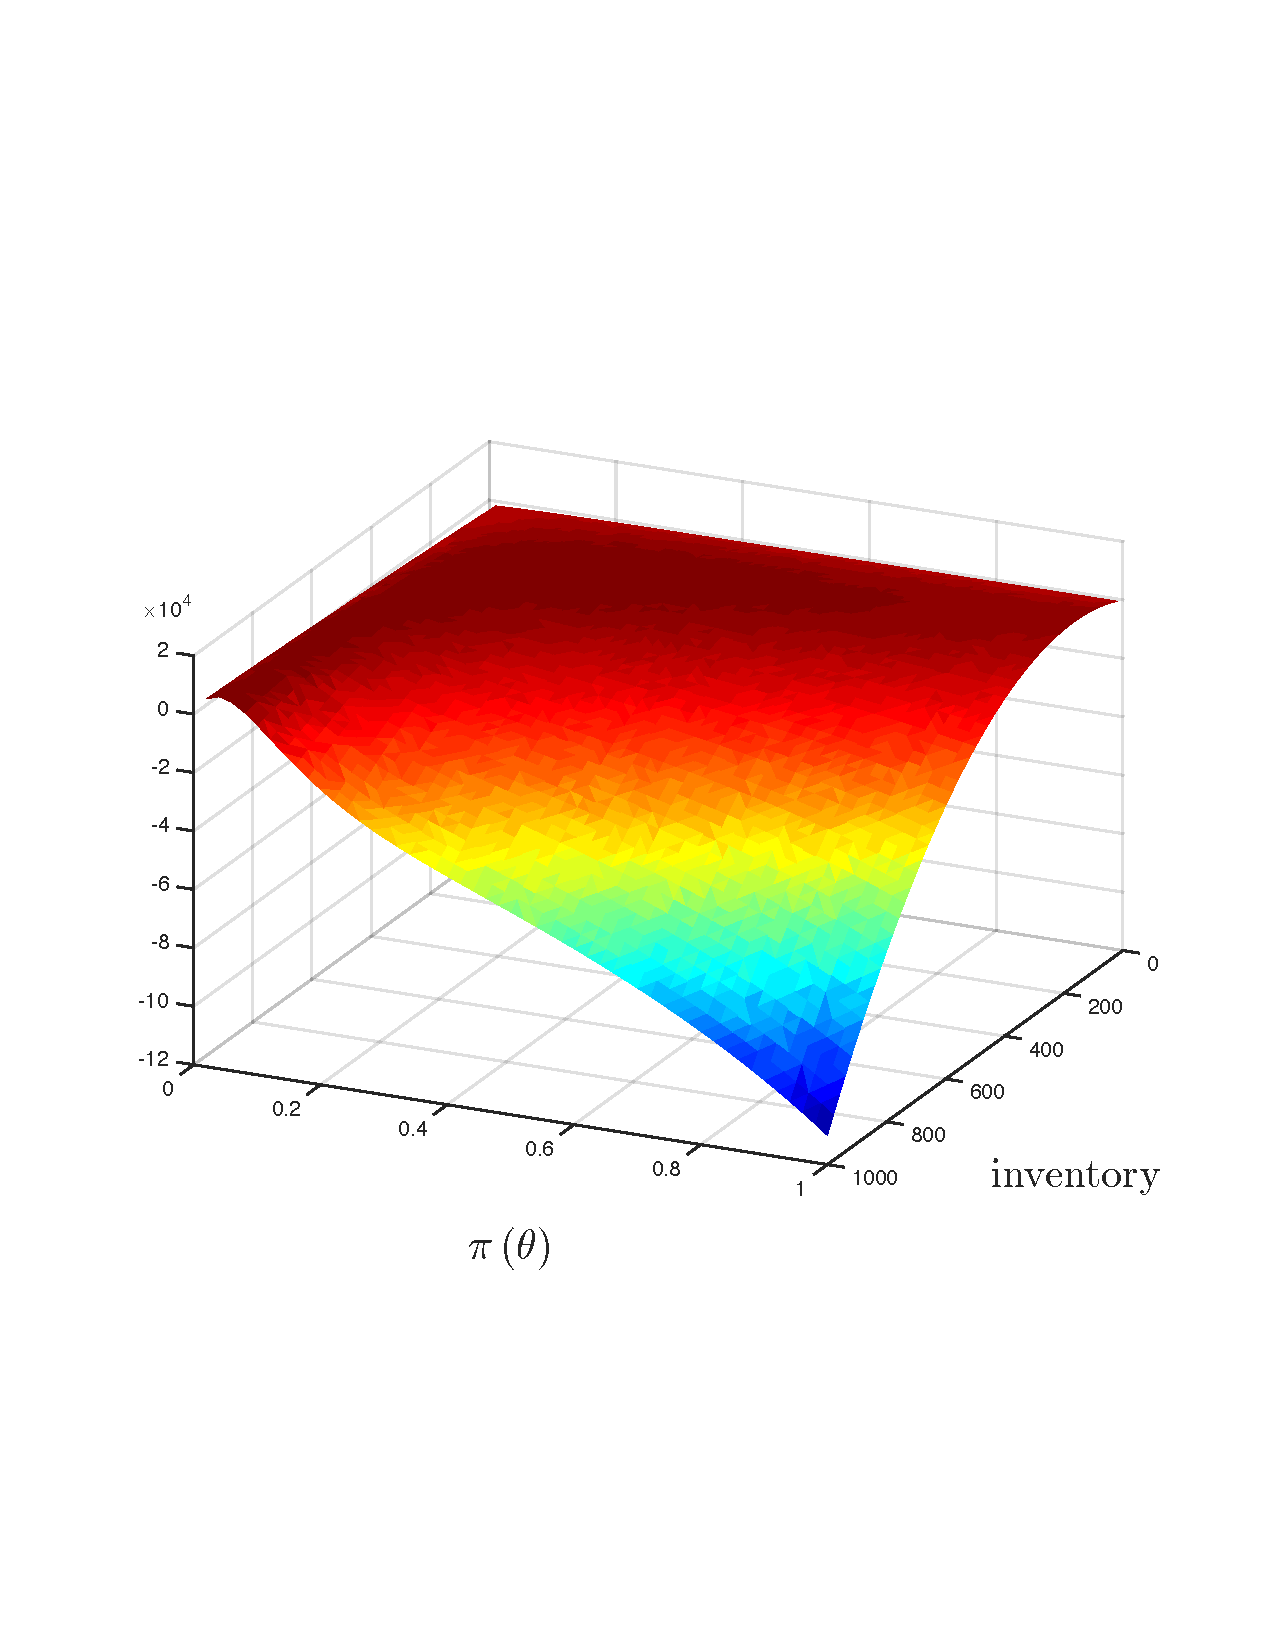
\includegraphics[width=\textwidth]{images/oe_vf_new}
                \caption{{\footnotesize $V^{\pi^{*}}(\theta, inv; \\\hspace{\textwidth}\qquad p = 55.0, \kappa = 0.165)$}}
                \label{fig:oe_vf}
                \end{subfigure}	&
            \begin{subfigure}{0.45\columnwidth}
                \centering
                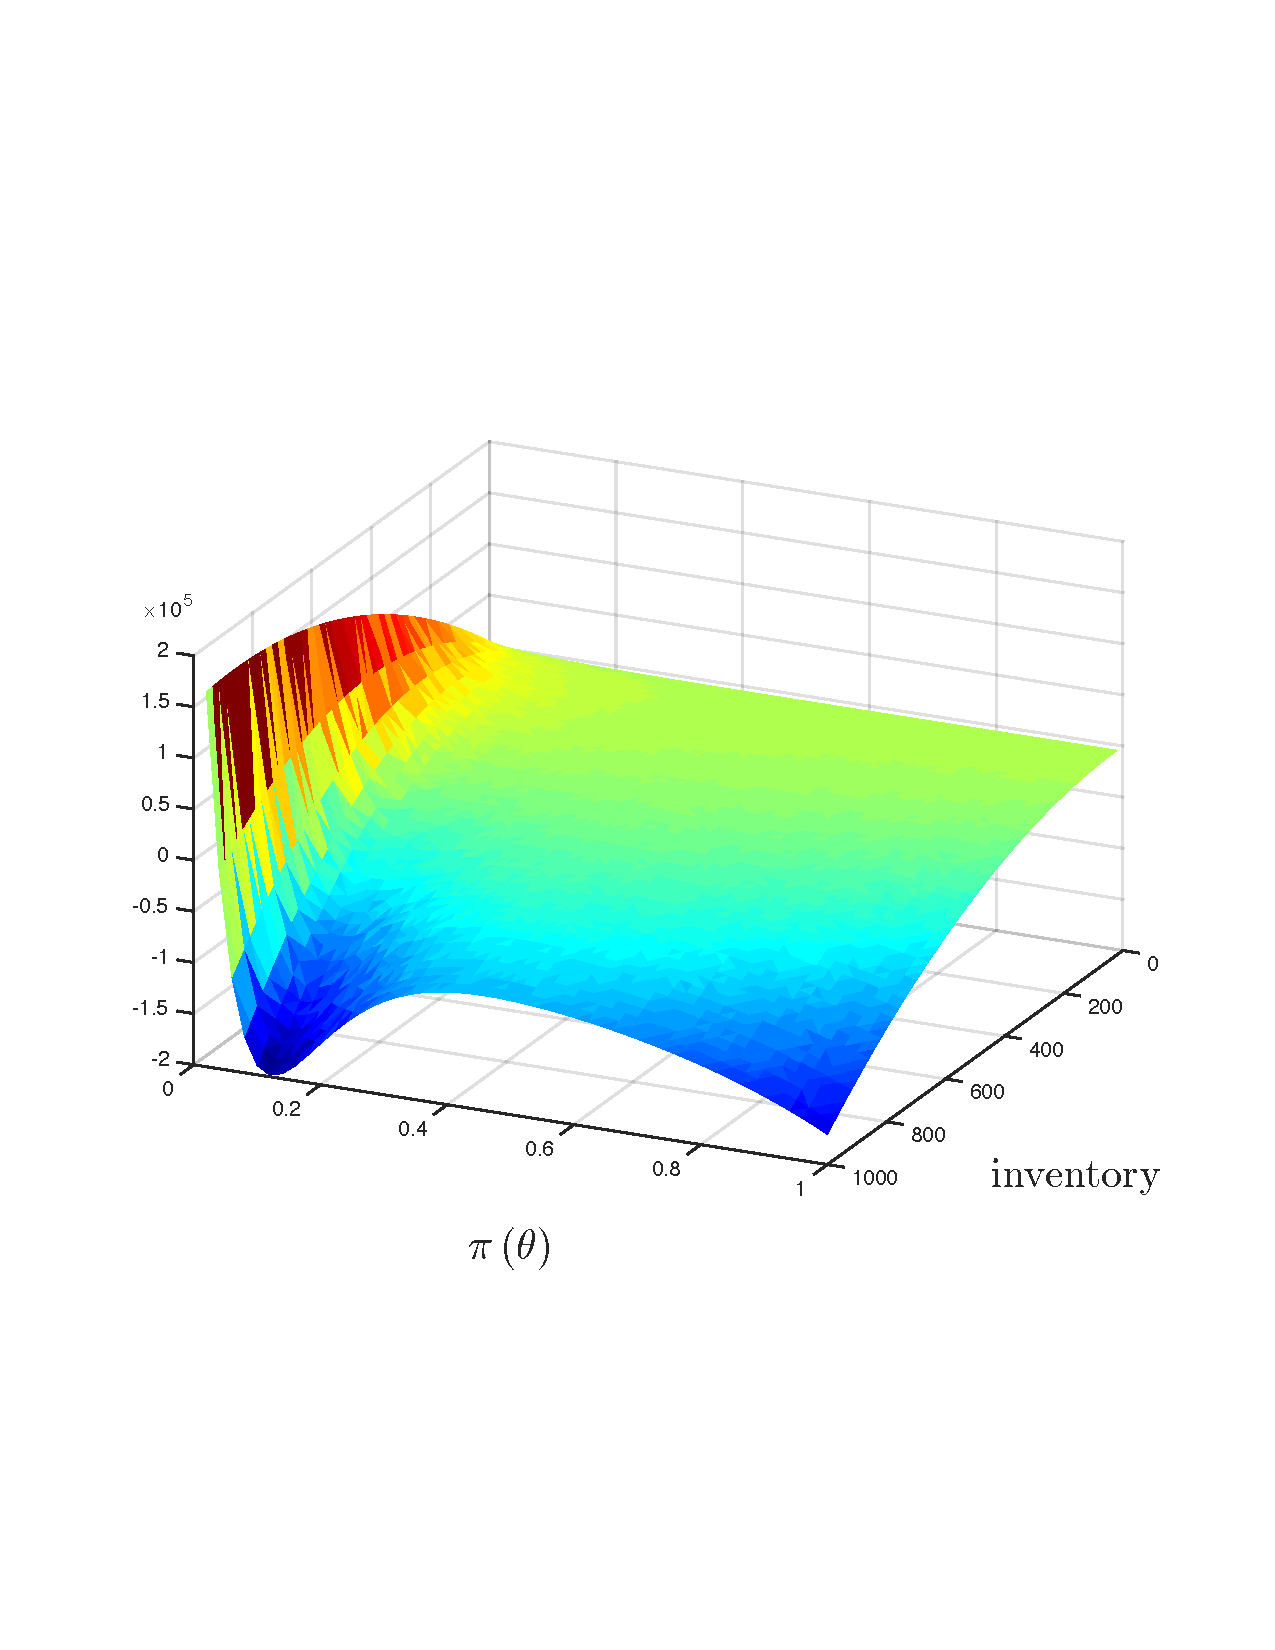
\includegraphics[width=\textwidth]{images/oe_vf_deriv_new}
                \caption{{\footnotesize $\nabla_{\theta} V^{\pi^{*}} (\theta, inv; \\\hspace{\textwidth}\qquad p = 55.0, \kappa = 0.165)    $}}
                \label{fig:oe_vf_deriv}
            \end{subfigure}
            \\            
        \end{tabular}
        \caption{Optimal Value functions for each domain.}        
        \label{tab:vf_Results}
%        \vspace{-3mm}
    \end{figure}
}

\subsection{SIR Epidemic}
\label{sec:results_influenza}

The well studied SIR epidemic~\cite{KermackMcKendrick_1927} domain is specified as follows: {\footnotesize $ \State = \left\langle s, i, r \right\rangle$}, where $ s $, $ i $, and $ r $ refer to the size of the susceptible, infected and recovered sub-populations, respectively. {\footnotesize $ \Action \in \left\lbrace \pi(\nu) \right\rbrace $} where {\footnotesize $\nu \in \left[0.0, 1.0\right]$} is the proportion of $ s $ to vaccinate at each stage. The transition function {\footnotesize \Transition} for each state variable in {\footnotesize \State} is given by:

{\footnotesize 
%    \abovedisplayskip=5pt
%    \belowdisplayskip=0pt
%    \renewcommand{\arraystretch}{1.5}
    \begin{tabular}{ll}
        $ \Transition\left( s' | s, i, r, \pi(\nu) \right) =$ & $ \delta \left[ s' - (s - \beta \cdot s \cdot i - \pi(\nu) \cdot s) \right] $ \\
        $ \Transition\left( i' | s, i, r, \pi(\nu) \right) =$ & $ \delta \left[ i' - (i + \beta \cdot s \cdot i - \lambda \cdot i) \right] $ \\
        $ \Transition\left( r' | s, i, r, \pi(\nu) \right) =$ & $ \delta \left[ r' - (r + \lambda \cdot i + \pi(\nu) \cdot s) \right] $ \\            
    \end{tabular}
}%
where {\footnotesize $ \beta $} is the infection rate and {\footnotesize $\lambda$} is the spontaneous recovery rate. The reward is specified as {\footnotesize $ \Reward\left(cost_{\mathtt{inf}}, cost_{\mathtt{vaccine}}, s, i, r, \pi(\nu) \right) = (s \cdot (-cost_{\mathtt{vaccine}} \cdot \pi(\nu) + (1 - \pi(\nu)))) - cost_{\mathtt{inf}} \cdot i + r$}. {\footnotesize $ cost_{\mathtt{inf}} $} is the incident cost of infection and {\footnotesize $ cost_{\mathtt{vaccine}} $} is the unit cost of vaccination. We assume that the total population is constant and that vaccinated individuals go straight from {\footnotesize $ s $} to {\footnotesize $ r $} without being infected. The decision maker must balance the cost of vaccination and the burden of disease on the population. 

Figure~\ref{fig:sir_vf} shows the optimal value function at {\footnotesize$ \Horizon = 7 $} when {\footnotesize $ s = 1000.0, i = 100.0, r = 0.0, \lambda = 0.25 $}, {\footnotesize $ cost_{\mathtt{vaccine}} = 4.0$} and {\footnotesize $ cost_{\mathtt{inf}} = 10.0 $}. The value function shows that it is not always optimal to vaccinate the entire population. In fact, Figure~\ref{fig:sir_opt} reveals that vaccinating the entire population is only optimal when {\footnotesize $ \beta > 0.25 $}, that is, when the \textit{basic reproductive ratio} {\footnotesize $ R_0 \,(= \beta/\lambda)$}~\cite{Heffernan_2005} exceeds 1.0. Scenarios where {\footnotesize $R_0 > 1.0$} can lead to an epidemic. 

To the best of our knowledge, this is the \textit{first} exact symbolic analysis of vaccination policies in an SIR model. Furthermore, PHMDPs and SDP can be used to solve \textit{any} SIR model without needing an analytical solution.

{\centering
    \begin{figure}[]
        \begin{tabular}{cc}
            \begin{subfigure}{0.45\columnwidth}
                \centering
                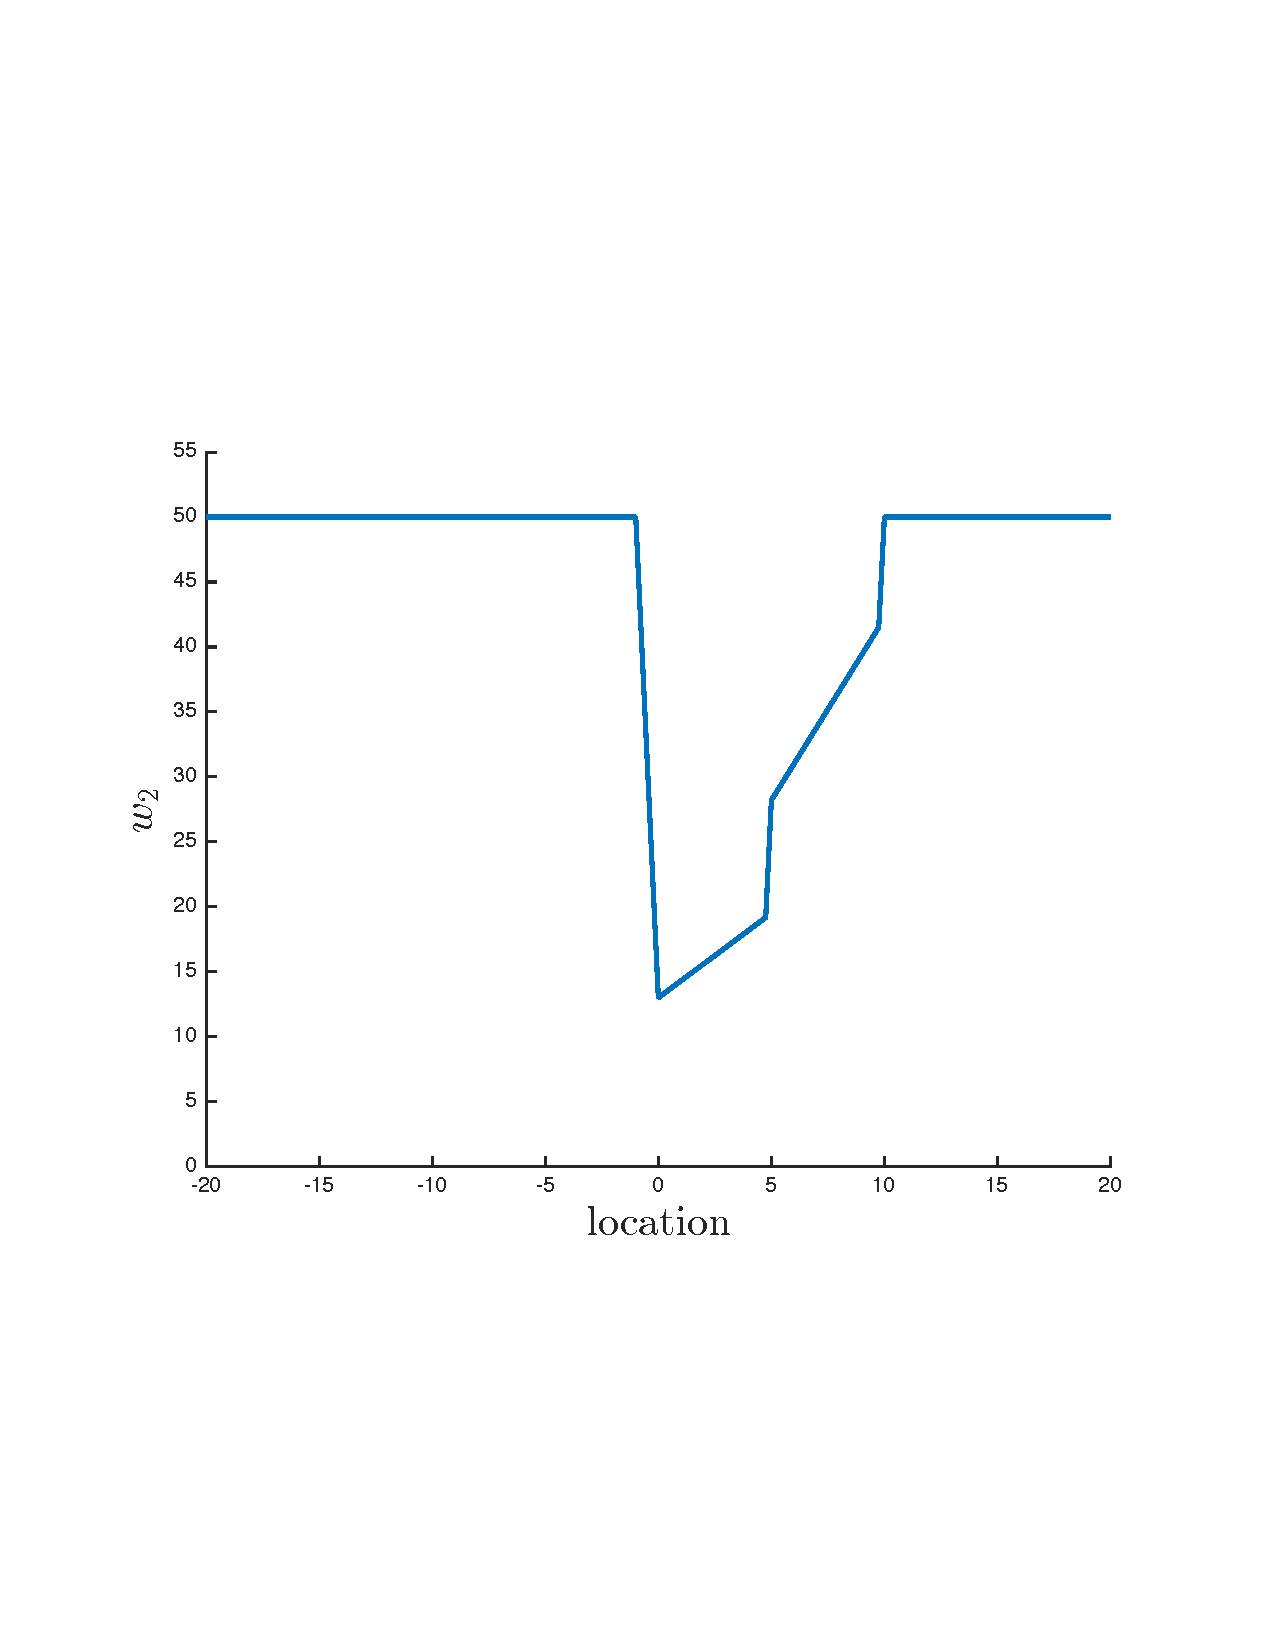
\includegraphics[width=\columnwidth,height=0.12\textheight]{images/robot_opt_new}
                \caption{Max {\footnotesize $w_2$} for $ \tilde{\pi} $}
                \label{fig:navigation_opt}
            \end{subfigure} &            
            \begin{subfigure}{0.45\columnwidth}
                \centering
                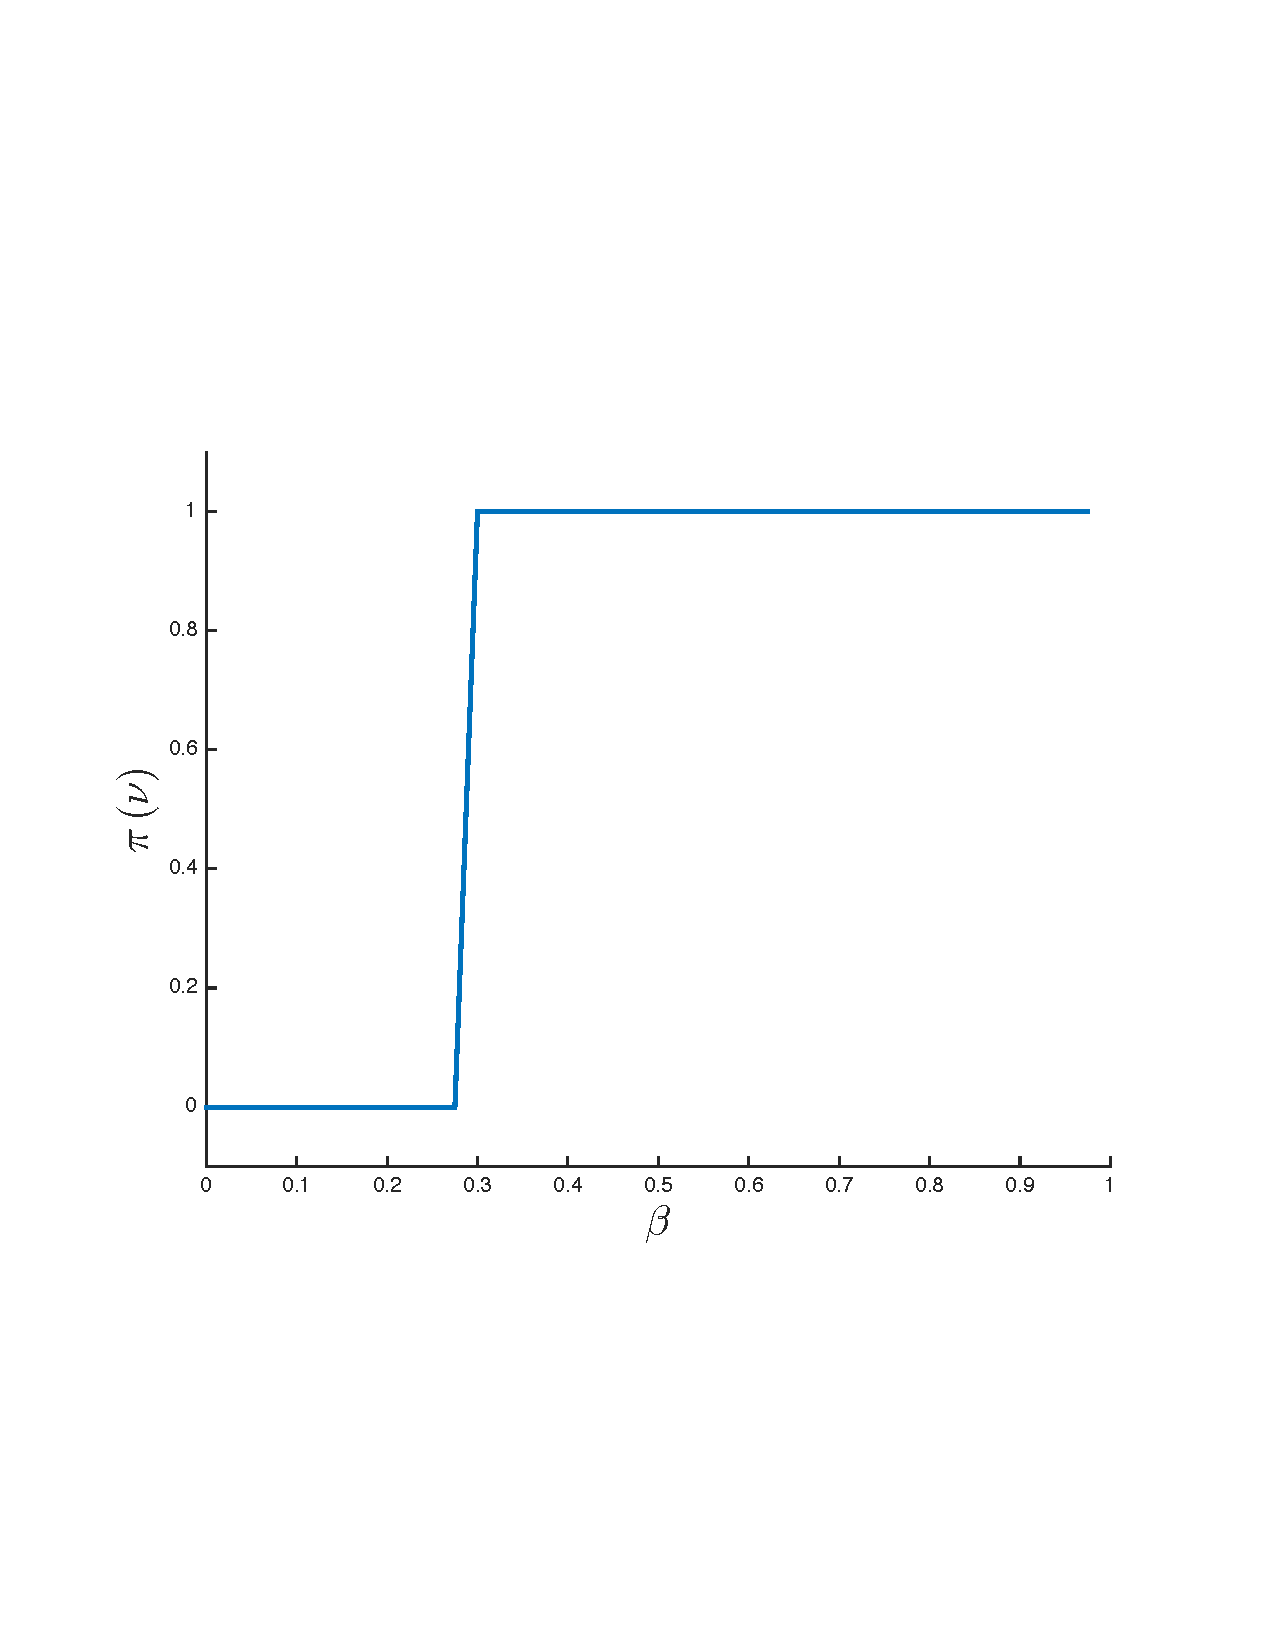
\includegraphics[width=\columnwidth,height=0.12\textheight]{images/sir_opt_new}
                \caption{{\footnotesize $ \pi(\nu) $} for {\footnotesize $ \beta \in \left[ 0.0, 1.0 \right] $}}
                \label{fig:sir_opt}
            \end{subfigure}
            \\
        \end{tabular}
        \caption{Nonlinear optimization for Navigation and SIR.}        
        \label{tab:opt_results}
%        \vspace{-3mm}
    \end{figure}
}

\subsection{Optimal Execution}
\label{sec:results_oe}

The domain is specified as follows {\footnotesize $ \State = \left\langle p, inv \right\rangle$}, where $ p $ is the price of the asset and $ inv $ is the inventory remaining. {\footnotesize $ \Action \in \left\lbrace \pi\left( \theta \right) \right\rbrace$}, where {\footnotesize $ \theta \in \left( 0.0, 1.0\right)$} is the proportion of inventory to be sold. The transition function {\footnotesize \Transition} for each state variable in {\footnotesize \State} is given by:

{\footnotesize 
%    \abovedisplayskip=5pt
%    \belowdisplayskip=0pt
%    \renewcommand{\arraystretch}{1.5}
    \begin{tabular}{ll}
        $\Transition\left( p' | p, inv, \pi\left( \theta \right) \right) =$ & $ \delta \left[ p' - (p - \kappa \cdot (inv \cdot \pi\left( \theta \right)) + \epsilon) \right] $ \\
        $\Transition\left( inv' | p, inv, \pi\left( \theta \right) \right) =$ & $\delta \left[ inv' - (inv - inv \cdot \pi\left( \theta \right)) \right] $ \\
    \end{tabular}
}%
where {\footnotesize $ \kappa > 0$} is a market-impact parameter and {\footnotesize $ \epsilon $} is a discrete noise parameter. The reward is specified by {\footnotesize $ \Reward\left(p', inv, \pi\left( \theta \right) \right) = p' \cdot inv \cdot \pi\left( \theta \right)$ }. 
When transacting a large number of shares, investors often face a trade-off between adverse market impact and the volatility of slow execution.

%Investors often face a trade-off between the adverse market impact of immediately transacting a large number of shares and the volatility of slow execution.

%market impact of transacting a large number of shares immediately and the volatility of slow execution. 

Figures~\ref{fig:oe_vf} and~\ref{fig:oe_vf_deriv} show the optimal value function at {\footnotesize $ \Horizon = 10 $} and its derivative w.r.t the parameter {\footnotesize $ \theta$}, respectively. When inventory is low, the value function is high at higher {\footnotesize $ \theta$} and the corresponding derivative is relatively stable. When the inventory is high, the value function is high at lower {\footnotesize $ \theta$} and the corresponding derivative shows maximum sensitivity. 
This indicates that when inventory is low, high {\footnotesize $\theta$} allows the investor to capture the current price and when inventory is high, lower {\footnotesize $\theta$} captures a more stable set of future prices. 
%This indicates that when inventory is low, selling a large proportion of shares allows the investor to capture the current price and when inventory is high, selling a lower proportion of shares captures a more stable set of future prices. 
\subsection{Time and Space Complexity}

\label{sec:time_space}

{\centering
\begin{figure}[]
    \begin{tabular}{cc}
        \begin{subfigure}{0.45\columnwidth}
            \centering 
            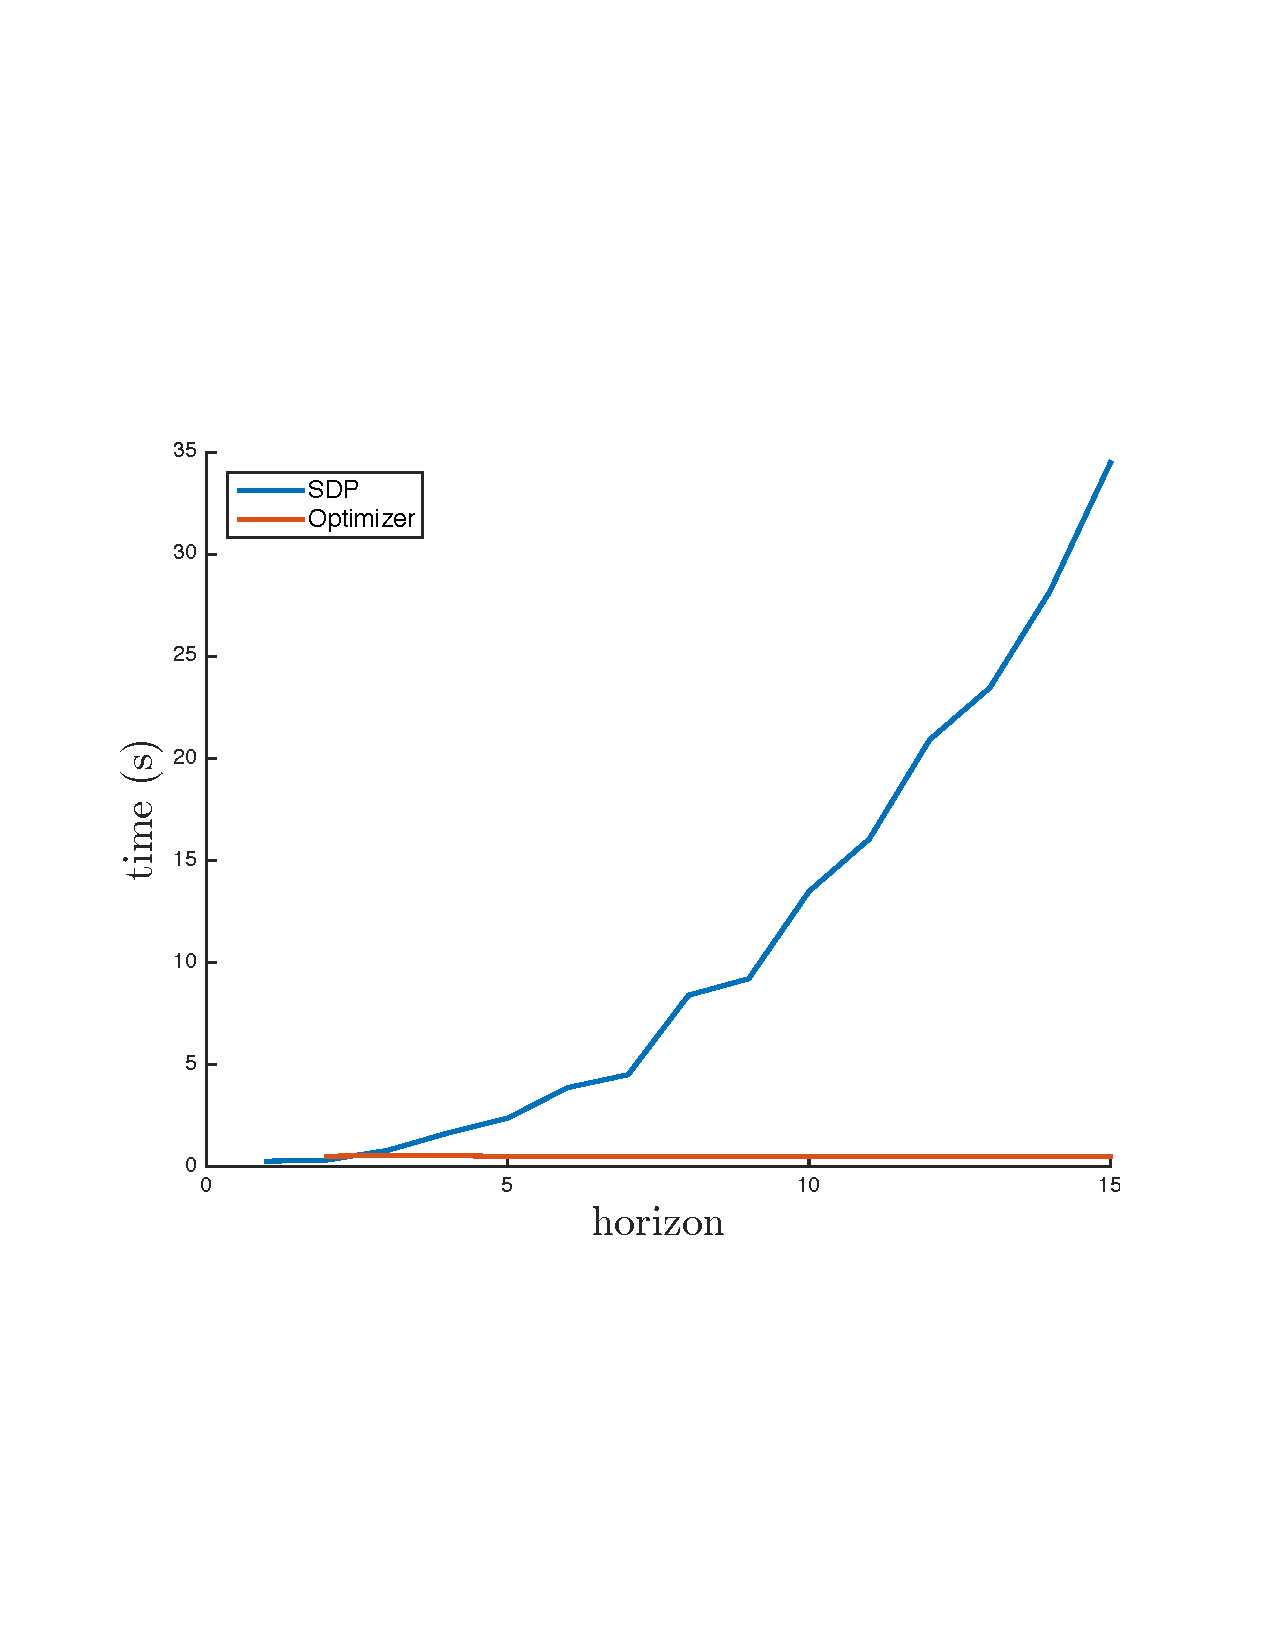
\includegraphics[width=\columnwidth,height=0.12\textheight]{images/time_plot_new}
            \label{fig:time_complexity}
        \end{subfigure} &
        \begin{subfigure}{0.45\columnwidth}
            \centering 
            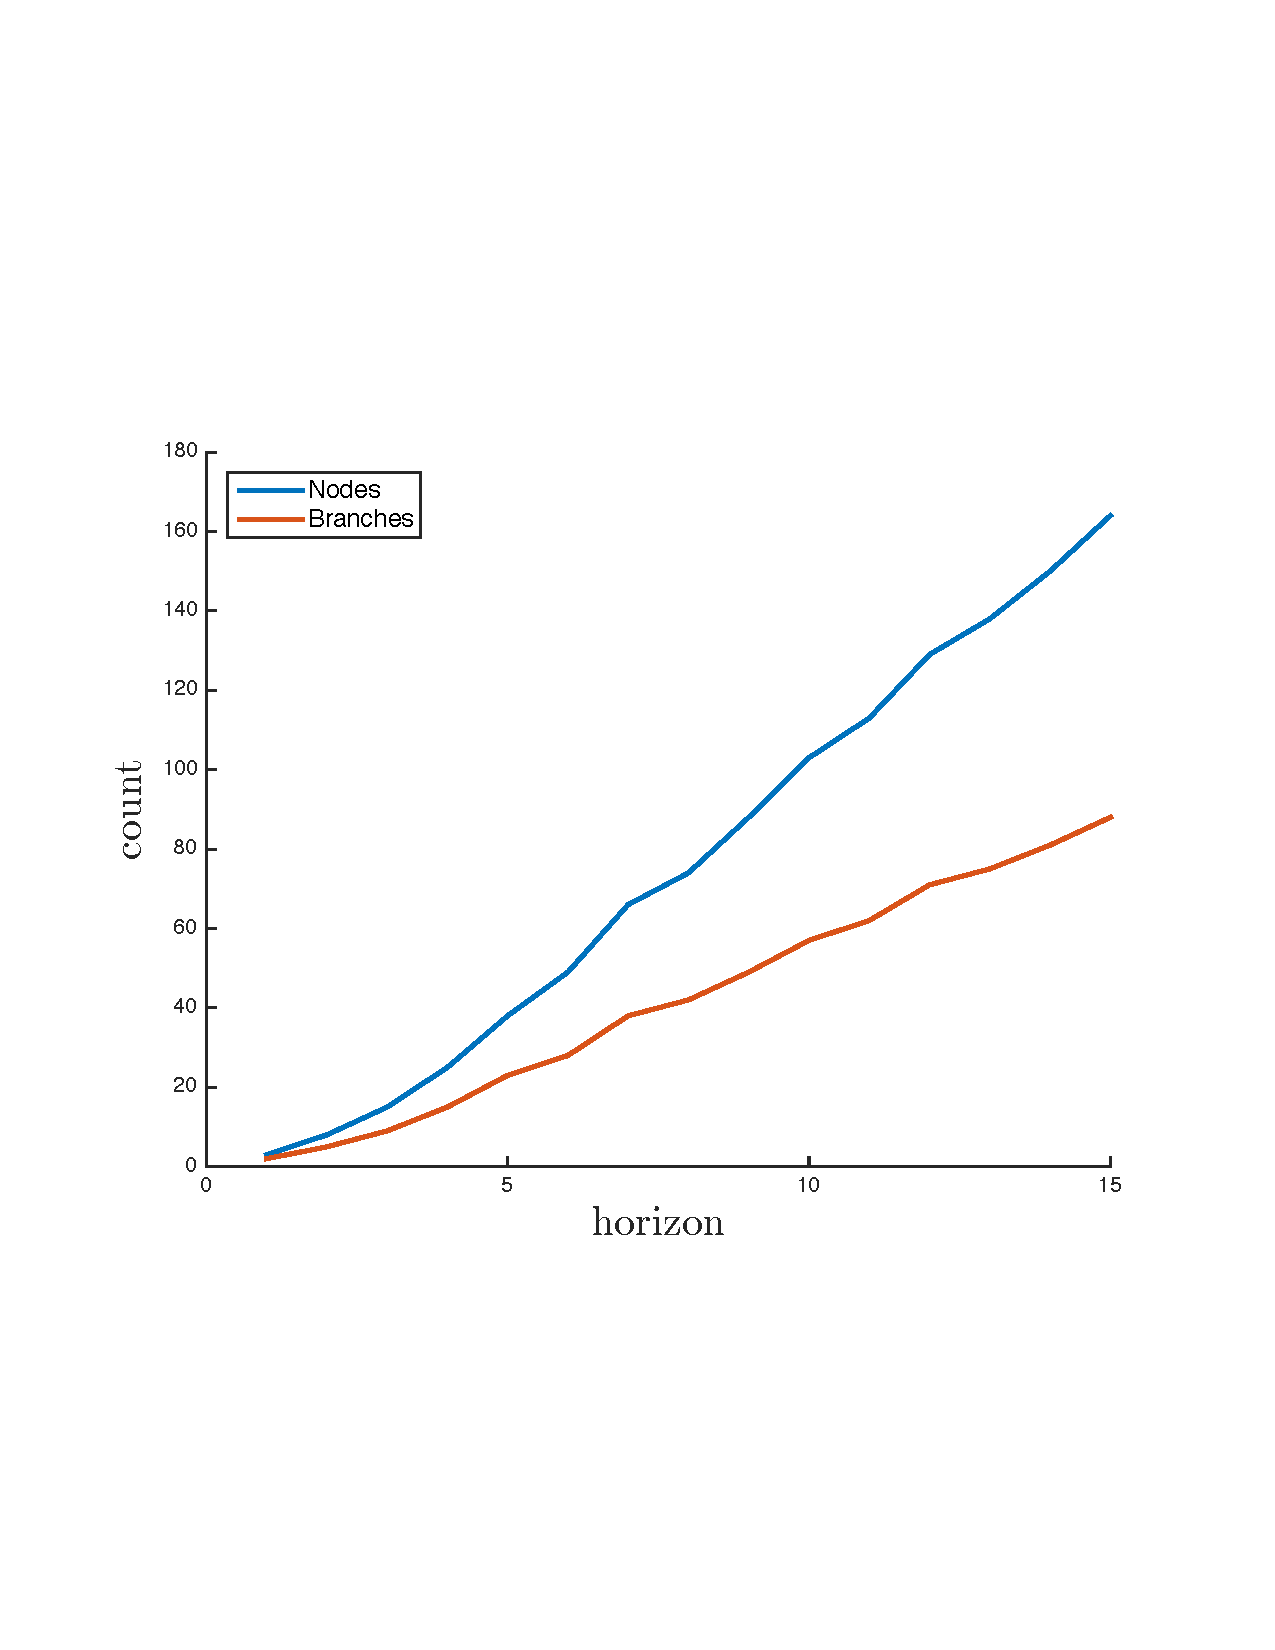
\includegraphics[width=\columnwidth,height=0.12\textheight]{images/space_plot_new}
            \label{fig:space_complexity}
        \end{subfigure}
        \\
    \end{tabular}
    \caption{Time and Space versus {\footnotesize $ \Horizon $} for Navigation.}
    \label{fig:time_space_complexity}    

\end{figure}
}

Figure~\ref{fig:time_space_complexity} shows an approximate linear relationship between the horizon {\footnotesize $ \Horizon $} and the computational time and space for the Navigation domain, which is a promising scalability property of the overall framework.

%--------------------------------------------------------------------------------------------------
% Bibliography
%--------------------------------------------------------------------------------------------------

% Bibliography
\bibliography{references}
\bibliographystyle{aaai}

\end{document}